% SIAM Article Template
\documentclass[review,onefignum,onetabnum]{siamart190516}
% SIAM Shared Information Template
% This is information that is shared between the main document and any
% supplement. If no supplement is required, then this information can
% be included directly in the main document.


% Packages and macros go here
\usepackage{lipsum}
\usepackage{amsfonts}
\usepackage{graphicx}
\usepackage{epstopdf}
\usepackage{algorithmic}
\ifpdf
  \DeclareGraphicsExtensions{.eps,.pdf,.png,.jpg}
\else
  \DeclareGraphicsExtensions{.eps}
\fi

% Add a serial/Oxford comma by default.
\newcommand{\creflastconjunction}{, and~}

% Used for creating new theorem and remark environments
\newsiamremark{remark}{Remark}
\newsiamremark{hypothesis}{Hypothesis}
\crefname{hypothesis}{Hypothesis}{Hypotheses}
\newsiamthm{claim}{Claim}

% Sets running headers as well as PDF title and authors
\headers{Application of semi-local sa to approximate pattern matching}{N. Mishin, and D. Berezun}

% Title. If the supplement option is on, then "Supplementary Material"
% is automatically inserted before the title.
\title{Application of semi-local sa to approximate pattern matching
  % \thanks{Submitted to the editors DATE.
  % \funding{This work was funded by the Fog Research Institute under contract no.~FRI-454.}}
}

% Authors: full names plus addresses.
\author{Nikita Mishin\thanks{Saint Petersburg State University, Russia
    (\email{mishinnikitam@gmail.com}).}
\and Daniil Berezun\thanks{IntelliJ Labs Co. Ltd., Saint Petersburg, Russia
  (\email{daniil.berezun@jetbrains.com}).}}

\usepackage{amsopn}
\DeclareMathOperator{\diag}{diag}


%%% Local Variables: 
%%% mode:latex
%%% TeX-master: "ex_article"
%%% End: 


% Optional PDF information
\ifpdf
\hypersetup{
  pdftitle={An Example Article},
  pdfauthor={D. Doe, P. T. Frank, and J. E. Smith}
}
\fi
\DeclareMathOperator*{\argmax}{arg\,max}
% The next statement enables references to information in the
% supplement. See the xr-hyperref package for details.

%\usepackage{algorithmic}
\externaldocument{ex_supplement}


\newcommand{\todo}[1]{{\color{red}TODO: {\color{blue}#1}}}
\newcommand{\Tau}{{\mathcal{T}}}

\newcommand{\red}[1]{\textcolor{red}{#1}}
\usepackage{interval}
\begin{document}

\maketitle

% REQUIRED
\begin{abstract}
  This is an example SIAM \LaTeX\ article. This can be used as a
  template for new articles.  Abstracts must be able to stand alone
  and so cannot contain citations to the paper's references,
  equations, etc.  An abstract must consist of a single paragraph and
  be concise. Because of online formatting, abstracts must appear as
  plain as possible. Any equations should be inline.
\end{abstract}


% REQUIRED
\begin{keywords}
  semi-local lcs, monge matrix, range queries, approximate matching, near-duplicate detection
\end{keywords}

% REQUIRED
\begin{AMS}
  68Q25, 68R10, 68U05
\end{AMS}

\section{Introduction}

% approximate string matching intro
The approximate pattern matching (\emph{AMatch}) is a well-known and studied problem.
Given some text $t$ and pattern  $p$ the \emph{AMatch} problem asks for all substrings of text $t$ that are close enough to pattern $p$ by some similarity measure.

% mant applications and difficulty
This problem arises in many fields such as computational biology, signal and image processing, text retrieval and etc \cite{}.
The diverse applications in sundry domains lead to different extensions of the problem which include additional constraints or even different objectives \cite{}.
Although there is a plurality of algorithms for solving the original \emph{AMatch} problem, the algorithm quantity dwindles notably when it comes to setting some constraints upon output.

The one such constraint naturally emerges and implicitly presented in various tasks\cite{TODO}. It refers to setting length bounds on matching substrings since minuscule or long matchings may be irrelevant to the subject of search (biologically insignificant, for example).
% Note that this constraint looks like

To the best of our knowledge, there is no formulation of extension of approximate pattern matching problem where the length of matchings explicitly limits, and, as consequences,  there is no study of this extended problem.

To close this gap, we take the liberty to define several extensions of \emph{AMatch} problem with explicitly set length constraint as well as provide algorithms for solving them. 
Recent achievements in RMQ in Monge matrices and novel \emph{semi-local lcs} problem is the key part of these algorithms.

We think that these problems with associated algorithms may be of practical use by virtue of natural constraints often occurring in different tasks.

In some ways, these algorithms are based on \cite{luciv2019interactive} algorithm.
In \cite{luciv2019interactive} the length constraint was given implicitly.
The algorithm is of interest not only because of the above limitation but also due to the fact that it satisfies some criteria of completeness that useful for some applications\footnote{the criteria is given in \cite{luciv2019interactive}}.
However, it has an unpleasant time complexity due to this limitation.

Taking into account the practical significance of \cite{luciv2019interactive}, we have developed an improved version of their algorithm with the perseverance of all of its properties based on the same concepts mentioned previously.

Thus, the main contribution of this paper is:
\begin{itemize}
    \item Improved version of the algorithm from \cite{luciv2019interactive}
    \item Definition and study of new extensions for  approximate pattern matching problem
    \item Algorithm for the new problem with an explicitly set length constraint on matching substrings 
\end{itemize}





% There also exist several variants of this problem that have different objectives with various implicitly or explicitly defined constraints.
% Although there are plenty of algorithms that solve \emph{AMatch} problem, the amount of algorithms significantly decreases when it comes to setting some constraints upon output. Nonetheless, recently, there was research in which the algorithm with implicitly defined length constraint was presented.
% This constraint was imposed on the lower and upper bound length of matching substrings.
% The algorithm is of interest not only because of the above limitation but also due to the fact that it satisfies some criteria of completeness that useful for some applications.
% However, it has an unpleasant time complexity.

% Taking into account the practical significance of this constraint in different tasks and domains we have developed an improved version of the algorithm [luciv] with the perseverance of all of its properties.
% This is achieved via adaptation and integration of algorithms that solve a novel string problem called "semi-local lcs problem".

% Further, we have defined a variant of \emph{AMatch} problem with explicitly set length constraint and presented exact and approximate algorithms for it.
% Recent achievements in RMQ in Monge matrices is the key part of these algorithms.

% Thus, the main contribution of this paper is:
% \begin{itemize}
%     \item Improved version of the algorithm from []
%     \item Algorithm for the new problem with an explicitly set length constraint on matching substrings 
%     \item Application of  "semi-local problem"
% \end{itemize}

\red{FILL WHEN OTHER PART IS READY}
The paper is orgranized as follows.

First, we give some basic definitions in section \ref{section:preliminaries}. Then, in  



% The length constraint of matching subsequences is an example of the latter one that often used in practice.
% It used in computational bioinformatics when the search  of a particular DNA subsequence in
% a large DNA sequence or DNA DATABASE is performed.
% Consider the case where we are given two matching substrings where the first one has a slightly higher similar score but has a significantly smaller size compared to the second one.
% There may be a situation when the application will yield only the first one substring although the second one may be more significant biologically.
% Thus, a specific lower bound on matching substrings should be set.

% Now consider the opposite case when the first one has a slightly smaller similar score but has a significantly smaller size compared to the second one.
% There could be a situation when the first one is much more significant in biology terms than the second one but the application will yield the second one. 
% Thus, a specific upper bound on matching substrings should be set.

% Same constraint arises in clone detection task when too small matching duplicates may be irrelevant  (article, interjections, punctuation marks, common words) whereas too big duplicates could not contains pattern at all (simply contains a word of pattern).


% The common approach of algorithm for approximate pattern matching utilizes  algorithm for solving the longest commons subsequence (\emph{LCS}) and sequence alignment (\emph{SA})  problems.

% The longest common subsequence is a well-known fundamental problem in computer science that also has many applications of its own.
% The major drawback of it that it shows only the global similarity for given input strings.
% For many tasks, it's simply not enough.
% The approximate matching is an example of it.

% There exist generalazation for \emph{LCS} called \emph{semi-local LCS}~\cite{tiskin2008semi} which can overcome this constraint. 
% The effective theoretical solutions for this generalized problem found applications to various algorithmic problems~\cite{tiskin2009periodic,tiskin2006longest,tiskin2011towards}.

% % research question Q1
% Although the algorithms for \emph{semi-local LCS} have good theoretical properties, there is unclear how they would behave in practice for a specific task and domain.
% More particularly, how it could be applied to approximate pattern matching with mentioned lower and upper bound on length constraint on matching subsequences.


% This paper is organized as follows

% % research question Q2
% To show the applicability of semi-local lcs on practice we developed several algorithms based mainly on it and the underlying algebraic structure.
% As well as developing new algorithms we improve the existing algorithm for duplicate detection in software documentation from~\cite{luciv2019interactive}.
% It should be noted that improvement preserves all properties of this algorithm.
% All presented algorithms also supports length constraints on the resulting substrings.
% Finally, we provided and proved running time and space complexity for all presented algorithms.





% Nonetheless, the number of suitable algorithms sharply decreases when the algorithm needs to meet some specific requirements imposed by running time, space complexity or specific criterion and constraints. 






% % short overview what constarins could be
% There exists a lot of algorithms that solve the above problem.
% Nonetheless, the number of suitable algorithms sharply decreases when the algorithm needs to meet some specific requirements imposed by running time, space complexity or specific criterion for the algorithm itself.
% For example, recently there was developed an approach for interactive duplicate detection for software documentation~\cite{luciv2019interactive}.
% The core of this approach is an algorithm that detects approximate clones of a given pattern $p$ with a specified degree of similarity and length boundaries for detected clones.
% The main advantage of the algorithm is that it meets a specific requirement of completeness.
% Nonetheless, it has an unpleasant time complexity.



   
% The common approach of algorithm for approximate detection utilizes mainly algorithm for solving the longest commons subsequence (\emph{LCS}) problem.

% The longest common subsequence is a well-known fundamental problem in computer science that also has many applications of its own.
% The major drawback of it that it shows only the global similarity for given input strings.
% For many tasks, it's simply not enough.
% The approximate matching is an example of it.

% There exist generalazation for \emph{LCS} called \emph{semi-local LCS}~\cite{tiskin2008semi} which overcome this constraint. 
% The effective theoretical solutions for this generalized problem found applications to various algorithmic problems~\cite{tiskin2009periodic,tiskin2006longest,tiskin2011towards}.
% %For example, there has been developed algorithm for approximate matching in the grammar-compresed strings~\cite{.}.

% % research question Q1
% Although the algorithms for \emph{semi-local LCS} have good theoretical properties, there is unclear how they would behave in practice for a specific task and domain.
% % research question Q2
% To show the applicability of semi-local lcs on practice we developed several algorithms based mainly on it and the underlying algebraic structure.
% As well as developing new algorithms we improve the existing algorithm for duplicate detection in software documentation from~\cite{luciv2019interactive}.
% It should be noted that improvement preserves all properties of this algorithm.
% All presented algorithms also supports length constraints on the resulting substrings.
% Finally, we provided and proved running time and space complexity for all presented algorithms.

% %% The paper is organized as follows.
% %% Blablabla
% %% \cref{sec:main}, our new algorithm is in \cref{sec:alg}, experimental
% %% results are in \cref{sec:experiments}, and the conclusions follow in
% %% \cref{sec:conclusions}.



\section{Preliminaries}
\label{section:preliminaries}

The section provides some backgraound, definitions, and theoremes required for
developed algortithms.

\subsection{Approximate pattern matching}
The approximate pattern matching problem ($AMatch$) defined as follows.
Given text $t$, pattern $p$, simularity function $g$, and some threshold $h$ the \emph{approximate pattern matching} problem asks for all substrings from text $t$ that have similarity score  with given pattern $p$ at least $h$ according to a function $g$.  

There exist different extensions and particular cases of the problem.
The most familiar case, \emph{complete approximate pattern matching} (\emph{CompleteAMatch}) that asks for all substrings of text $t$ that are exact clones of pattern $p$.
CompleteAMatch can be solved by a number well-knonwn algorithms such as Aho--Korasic, Bouer--Murr, Knuth--Morris--Pratt, and so on.
The optimal CompleteAMatch solution running time is $O(|p|+|t|)$~\cite{.}.
Other special cases of AMatch are \emph{approximate pattern matching with k mismatches}~\cite{.}, search of \emph{pattern with wildcard symbols}~\cite{.}, multidimensional \emph{AMatch}~\cite{.}, AMatch with a length constraint on the resulting substrings~\cite{.}, and many more~\cite{.}.

One of the common approaches to solving AMAtch problem is the utilization of string similarity problem solutions.
Latter represents a set of fundamental problems such as \emph{edit distance}, \emph{longest common subsequence}, and \emph{sequence alignment}.
\todo{In the paper, we primarily focus on the usage of the latter two when developing algorithms.}

Recently there has been developed an algorithm for solving one particular \emph{AMatch} extension~---~the one with a length constarint on the resulting substrings~\cite{.}.
\todo{Describe why the problem is actual}.
Despite the algorithm \todo{has poor result in terms of running time complexity}, the proposed solution possesses a completeness property, i.e it founds \emph{all} non-intersected clones of a given pattern with specified similarity threshold and length constraint on matching substrings.
Precisely due to the completeness property the algorithm is of intereset in this paper.
The algorithm is described in section~\ref{.} while the developed improved version is presented in section~\ref{.}.

\subsection{Global lcs and sa}
% Semi-local lcs and sa are extensions of \emph{lcs} and \emph{sa} problems, respectively.

\begin{definition}
Given two strings $a$ and $b$  the longest common subsequence (\emph{LCS}) problem ask for the maximal length of the longest common subsequence of $a$ and $b$ ($lcs(a,b)$).
\end{definition} 
\todo{In other words, \emph{LCS} problem asks about maximal $lcs$ score of two given string $a$ and $b$ ($lcs(a,b)$)}.

\begin{definition}
Given two strings $a$ and $b$ and scoring scheme $w=(w_{+},w_{0},w_{-})$ the sequence alignment (\emph{SA}) problem ask for the maximal alignment score between $a$ and $b$ ($sa(a,b,w)$).
\end{definition}

Scoring scheme determines how to calculate the alignment score of two aligned sequences.
If a pair of character in aligned sequences are matched (equal) then this pair contributes to the final alignment score $w_{+}$, if their mismatch it contributes $w_{0}$.
If symbol $\alpha$ of one of the sequences is not aligned with any other symbol from another sequence it means that $\alpha$ is aligned with a $gap$.
In this case, this pair contributes $w_{0}$.
The final scoring scheme calculates as follows:
\begin{equation}\label{formula:sa}
\begin{array}{ll}
    sa(a,b,w) &= w_{+}k^{+} + w_{0}k^{0} + w_{-} (|a| + |b| - 2k^{+} - 2k^{0}) \\
    &= k^{+} (w_{+} - 2w_{-} ) + k^{0}  (w_{0} - 2w_{-}) + w_{-}(|a| + |b|)
\end{array}
\end{equation}
where $k^{+}$ stands for the number of matched symbols, $k^{-}$ --- the number of mismatched symbols.
Note that \emph{LCS} is a special case of \emph{SA} with scoring scheme be $(1,0,0)$.
Both described problems can be solved with usual dynamic programming algorithm having running time complexity $O(|a|\times|b|)$.

\subsection{Semi-local lcs}

$LCS$ and $SA$ allow one to find how much whole given strings are similar, i.e. how similar two string in a global sense.
Sometimes this is not enough.
There exist \emph{fully local} and \emph{semi-local} generalizations of these problems.
In the paper, we focus on \emph{semi-local} ones due to natural applicability to approximate pattern matching.
The key feature of semi-local problems is that they can be solved within the same time as global ones while collects more information about strings similarity.
More precisely, given two strings $a$ and $b$ the semi-local lcs asks about $lcs$ scores for following:
\begin{itemize}
\item \emph{string-substring}: whole $a$ against every substring of $b$,
\item \emph{substring-string}: whole $b$ against every substring of $a$,
\item \emph{prefix-suffix}: every prefix of $a$ against every suffix of $b$,
\item \emph{suffix-prefix}: every prefix of $b$ against every suffix of $a$.
\end{itemize} 
Formally, semi-local lcs can be defined via \emph{semi-local lcs matrix} as follows.
\begin{definition}
The \emph{semi-local lcs matrix}  $H_{a,b}$ for strings $a$, $b$ defined as follows:
\begin{equation}
  H_{a,b}[i,j] = \textbf{ if } j\leq i \textbf{ then } j-i \textbf{ else } lcs(a,b^{pad}[i,j]) 
\end{equation} 
where $i \in [-|a|:|b|], j \in [0:|a|+|b|] $, $b^{pad}= ?^{|a|}\ b\ ?^{|a|}$, $?$--- wildcard symbol that matches any other symbol.
\end{definition}
The semi-local lcs matrix $H_{a,b}$ comprises from four quadrants associated with described subproblems:
\begin{equation}
  H_{a,b} = \begin{bmatrix}
    H_{a,b}^{suf-pre} & H_{a,b}^{sub-str} \\
    H_{a,b}^{str-sub} & H_{a,b}^{pre-suf} 
  \end{bmatrix}    
\end{equation}

\subsection{Matrix properties}

\begin{definition}
Matrix $H$ called (anti) Monge matrix if

\begin{displaymath}
  \forall i,i',j,j':\ i\leq i^{'}, j \leq j^{'}\ .\ H[i,j]+H[i^{'},j^{'}] (\geq)\leq H[i,j^{'}]+H[i^{'},j]
\end{displaymath}
\end{definition}

\begin{definition}
Let $H[0:m,0:n]$  be a matrix.
$H^{\square}[0:m-1,0:n-1]$ constructed as a result of taken cross difference between secondary and first diagonal for all adjacent 2 by 2 squares called \emph{cross-difference} matrix of  $H$
\end{definition}


\begin{definition}
Matrix $H$ called unit anti Monge matrix if $H$ is (anti) Monge matrix and its \emph{cross-difference matrix} $(-)H^{\square}$ is permutation matrix.
\end{definition}
The example of unit anti Monge matrix is following:
\begin{equation}
\begin{bmatrix}
0 & 2 & 3 \\
0 & 1 & 2 \\
0 & 1 & 1
\end{bmatrix} ^ { \square} =
\begin{bmatrix}
(2 + 0) - (1 + 0)  & (3 + 1) - (2 + 2)  \\
(1 + 0) - (1 + 0) &  (2 + 1) - (1 + 1) 
\end{bmatrix} = 
\begin{bmatrix}
1 & 0  \\
0 & 1 
\end{bmatrix} 
\end{equation}
 
\begin{definition}
Let $H[0:m-1,0:n-1]$  be a matrix.
$H^{\nearrow}[0:m,0:n]$ constructed as sum of element that lies below and left given cell $i,j$ in matrix $H$ called \emph{dominance-sum} matrix of $H$
\end{definition}

The example dominance sum matrix:
\begin{equation}
\begin{bmatrix}
1 & 0  \\
0 & 1 
\end{bmatrix}^{\nearrow} =
\begin{bmatrix}
0+0+0 & 1 & 1+1 \\
0+0 & 0 & 1 \\
0 & 0 & 0
\end{bmatrix} =
\begin{bmatrix}
0 & 1 & 2 \\
0 & 0 & 1 \\
0 & 0 & 0
\end{bmatrix}
\end{equation}

In~\cite{tiskin} is proved that $H_{a,b}$ is unit anti Monge.
Also, it is proved that this matrix may be decomposed to permutation matrix, i.e into a \emph{cross-difference} matrix.
It allows to store $H_{a,b}$ implicitly and query any element of $H_{a,b}$ via dominance sum query (orthogonal range queries).
Thus, there are several ways to store matrix $H_{a,b}$ or one of its quadrants implicitly.
A simple storing of two lists of permutations requires $O(|a|+|b|)$ space and time \todo{with $O(|a|+|b|)$} orthogonal range queries (need to check how many points dominated by given point), whereas more sophisticated approach requires $O(|a|+|b|)$  space with $O( (|a|+|b|) \sqrt{\log{ (|a| +|b|)} } )$ preprocessing time and allows to query any point of $H$ in $O(\frac{\log (|a|+|b|)}{\log \log (|a|+|b|)})$ time.  

\todo{The one useful proposition of $H$ is the following}~\cite{.}.
\begin{proposition}
  Given a permutation matrix $P$ and a value $P^{\nearrow}[i; j]$,
  values $P^{\nearrow}[i +- 1; j], P^{\nearrow}[i; j +- 1]$, where they exist,
  can be queried in time $O(1)$.
\end{proposition}

We particularly interested in the left lower quadrant that refers to string-substring problem:
\begin{equation}
H_{a,b}^{str-sub}[i,j] = lcs(a,b[i,j]) \quad i,j \in [0,|b|] 
\end{equation}

\todo{There exists several algorithms \red{second on,recursive not described as i see} that solve \emph{semi-local lcs}.
Both have the optimal running time $O(|a| \times |b|)$ for given dynamic problem\cite{}\red{Impossibility faster then pt}.}

\subsection{Semi-local sa}
The semi-local sequence alignment is a generalization of semi-local lcs in the same manner as sequence alignment is a generalization of lcs.
Given two strings $a$ and $b$ and scoring scheme $w=(w_{+},w_{0},w_{-})$  semi-local sa asks about sa scores for the following:
\begin{itemize}
\item \emph{string-substring}: whole $a$ against every substring of $b$
\item \emph{substring-string}: whole $b$ against every substring of $a$
\item \emph{prefix-suffix}: every prefix of $a$ against every suffix of $b$
\item \emph{suffix-prefix}: every prefix of $b$ against every suffix of $a$
\end{itemize} 
The \emph{associated matrix} for semi-local sa is defined by analogy as for semi-local lcs.

Semi-local sa problem can be solved by reducing to semi-local lcs.
First, note that the scoring scheme from~\ref{formula:sa} may be simplified by so-called normalization~\cite{.}:\todo{check equation}
\begin{equation}\label{weightNormalization}
  \begin{array}{ll}
    w &= (w_{+}, w_{0} , w_{-}) \xrightarrow{} (w_{+} +2x , w_{0} + 2x , w_{-} + x)\\
    &= ( \frac{w_{+} +2x}{w_{+} +2x} , \frac {w_{0} + 2x}{w_{+} +2x} , \frac{w_{-} + x}{w_{+} +2x})_{x=-w_{-}} = (1,\frac{\mu}{v} ,0) 
  \end{array}
\end{equation}
The resulted scoring scheme $w_{normalized} = (1,\frac{\mu}{v} ,0)$ is called the \emph{normalized scoring scheme}.
Then to query initial score $sa$ for scoring scheme $w$ knowing $sa_{normalized}$ for $w_{normalized}$ one need to apply reverse regularization:
\begin{equation}
  \begin{aligned}
    sa(a,b,w) = sa_{normalized}  (w_{+} - 2w_{-}) +  w_{-} (|a| + |b|)
  \end{aligned}
\end{equation}

Finally, the blown-up technique is applied after reducing scoring scheme which increases both input strings in $v$ times.
\todo{Nonetheless, only one of the described algorithm time complexity increases in $v^{2}$ times, the second one only $v$. \red{Bad sentecnce}.
The space complexity also increses by factor $v$. }
%(we store permitation matrix of size $(v(|a|+|b|) \times v(|a|%%+|b|) $) 
%Thus, the rinning time and space complexity of semi-local sa is %$(v(|a|+|b|) \times v(|a|+|b|) $ and 
\todo{The detalied description can be found in TISKIN BOOK~\cite{.}.}

 
\subsection{Range maximum/minimum queries}

Range maximum/minimum queries (\emph{rmq}) (submatrix query)  refers to search maximum/minimum element in submatrix $[i_{1}:i{_2}]\times [j_{1}:j{_2}]$ of given matrix $M$ of size $n\times n$.
The associated data strucutre that can report maximum/minimum element in any  submatrix query called \emph{range maximum/minimum data structure}.

For the generic case of Matrix $M$ it is not possible to
achieve running time faster then $O(n^2)$ due to fact that storing matrix $M$ requires $O(n^2)$.

Nonetheless, the situation is changed if we  consider special cases such as Monge matrices.
%Monge matrices can  be (and often) stored implicilty.
There have been several researches over several decades about 
rmq on monge matrices \cite{}.

The recent research achives following result\cite{}.

\begin{theorem}\cite{}
Given an $n \times n$ Monge matrix $M$, a data structure of size $O(n)$ can be constructed
in $O(n \log n)$ time to answer submatrix maximum queries in $O(\log \log n)$ time when random access to Monge matrix is $O(1)$.
\end{theorem}


\begin{theorem}\cite{}
Given an $n \times n$ staircase\footnote{Defintion} Monge matrix $M$, a data structure of size $O(n)$ can be
constructed in $O(n \log n$) time to answer submatrix maximum queries in $O(\log \log n$) time when random access to Monge matrix is $O(1)$.
\end{theorem}


\begin{theorem}\cite{}
Given an $n \times n$ partial Monge matrix\footnote{Definition} $M$, a data structure of size $O(n)$ can be
constructed in $O(n \log n$) time to answer submatrix maximum queries in $O(\log \log n$) time when random access to Monge matrix is $O(1)$.
\end{theorem}

The above results applies both to range  minimum queries and to monge matrices with non-constant access $O(\beta)$ to queries.
The latter one, costs in  increased construction time and query time by factor $\beta$. 

  
%\begin{definition}
%Given  query of type $i_{1},i_{2},j_1,j_2, i_1,i_2 \in [0,]$
%\end{definition}
%\emph{rmq}  





\subsection{Near-duplicate detection algorithm}
First, we denote several parameters, that is used in algorithm \cite{}.
$k$--- constant in interval $[\frac{1}{\sqrt{3}},1]$ that set similarity measure.  
A window $w$ of size $L_{w} = |p|/k$ is to process text $t$ with
sliding window of one symbol step.
$k_{di} = |p|*(\frac{1}{k}+1)(1-k^2)$ is threshold value for edit distance.
$I$ --- interval of size $[|p|k,\frac{|p|}{k}]$ that set boundaries for lenght of matching substrings.
$d_{di}$ --- function that measure similarity between two strings.

The algorithm comprises of three phases.

At the first phrase  text $t$ is processed with sliding window of size $L_{w}$ with one symbol step.
Further, substrings that corrsepond to window $w$ compared using edit distance\footnote{Authors of \cite{} used lcs edit distance --- where  operations substituion,removoval, addition of one symbol costs 2,1,1 respectively} and if $d_{di}(p,t_{w}) \leq k_{di}$ i.e  close enough, then they saved to set $W_{1}$ to be further proceeded. 

On the second phase  each of the detected substrings in $W_{1}$ are shrunk i.e they lenght could be decreased.
More preciesely, within each of the element of $W_{1}$ the largest one substring with legnth fall in $I$ that most similar to pattern $p$ according to $d_{di}$ is selected.
The set $W_{2}$ is a result of this phase.

At the final third phase  set $W_{2}$ iterated over to remove elements that fully contains in ohter elements of $W_{2}$ or duplicates.


\begin{algorithm}[H]
\caption{PATTERN BASED NEAR DUPLICATE
SEARCH ALGORITHM}\cite{}
\label{alg:luciv}
Input: pattern $p$, text $t$, $k$ ---similiarity measure\\
Output: Set of non-intersected clones of pattern $p$ in text $t$\\
Pseudocode:
\begin{algorithmic}[1]
\STATE{$W_1 = \emptyset$}
\COMMENT{1st phase}
\FOR{$\forall w_{1}:w_{1} \in t \land |w_{1}|=L_{w} $}
\IF{$d_{di} \leq k_{di}$}
\STATE{add $w_1$ to $W_{1}$}
\ENDIF
\ENDFOR
\STATE{$W_{2} = \emptyset$}
\COMMENT{2d phase}

\FOR{$w \in  W_{1}$}
\STATE{$w^{'}_{2} = w$}
\FOR{$l \in I $}
\FOR{$\forall w_2: w_2 \subseteq  w \land |w_2| = l$} 
\IF{$Compare(w_{2}, w_{2}^{'},p)$}
\STATE{$w_{2}^{'} = w_2$} 
\ENDIF
\ENDFOR
\ENDFOR
\STATE{add $w_{2}^{'}$ to $W_{2}$}
\ENDFOR

\STATE{ $W_3 = UNIQUE(W_2)$}

\COMMENT{3rd phase }
\FOR{$w \in W_3$}
\IF{$\exists w^{'} \in W_3:w \subset w^{'} $}
\STATE{ $remove$ $w$ $from$ $W_3$}
\ENDIF
\ENDFOR
\RETURN $W_3$

\end{algorithmic}
\end{algorithm}

\paragraph{Running time analysis}
\emph{1st phase}.The first phase requires at most  $O(|t||p|^2)$ due to fact
that computing cost of edit distance is $|p|^2$ for strings of size $O(|p|)$ and we need to process $O(|t|-\frac{|p|}{k})=O(|t|)$ windows.
\emph{2nd phase}. 
The cardinality of set $W_{1}$  at worst case be $O(|t|)$.
Thus, first loop will be iterated over $O(|t|)$ times.
The second loop refers to iteration over $I$ set with cardinality $O(\frac{|p|}{k}-|p|k) = O(|p|)$.
The third loop requires at most $O(|p|)$ since we again goes with sliding window.
The compare operation requires at most $O(|p|^2)$ since both
stirng of size $O(|p|)$.
Thus, the total running time compleixty of second phase is $O(|p|^4|t|)$ at worst case.

\emph{3rd phase}. 
Note that cardinality of set $W_{2}==W_{1}$ and thus at worst case is $O(|t|)$.
Then, this phase requires $O(|t| \log |t|)$ time. 

Thus,the total time complexity of algirthms estimates as 
$O(max(|t||p|^4,|t| \log|t|))$.

Algorithm also possesses completnesses property defined in their paper. 
To detailed description refer to \cite{}.
We just state their following theorem:
\begin{theorem}\cite{Luciv}
For any $p \in t$ , $k \in (\frac{1}{ \sqrt{3}} , 1]$ and near
duplicate group $G$ of fragment $p$ with similarity $k$ the criterion of \emph{completeness} is satisfied in
respect to the output of phase 2.
\end{theorem}

Theorem states that if pattern $p$ is presented in text $t$ then all duplicates of it would be found in text $t$. 

\section{Algorithm for near duplicate detection}
\label{section:luciv}

In the section the improved version of Luciv et.al. algorithm~\cite{luciv2019interactive} is presented.
The utilization of semi-local sequence alignment algorithms in algorithm phases improves overall time complexity.
%% We now describe an improved version of  by utilizing a \emph{semi-local sa} solution.
%% Then we present proof that improved version preserves completnesess property.
%% It is achieved by imitating all phases of the algorithm. 
It is also proved that the improved algorithm preserves all advantages of the initial one stated at~\cite{luciv2019interactive} such as search completeness.

\subsection{Algorithm description}
As the base one (see section~\ref{sec:lucivalgo} and~\ref{Luciv}), the presented algorithm consists of three sequential phases.
%Moreover, each step of the presented algorithm imitates the corresponding step of the base one.
Aldorithm pseudocode is presented at Algorithm~\ref{alg:patternMathing1}.
% As the base one, the presented algorithm comprises three phases.

At the first phase (lines 1-3) semi-local sa problem is solved for pattern $p$ against the whole text $t$.
This solution provides access to the string-substring matrix $H^{str-sub}_{p,t}$ which allows performing fast queries of \emph{sa} score for pattern $p$ against every substring of text $t$.
Then, we construct matrix $M$ by applying transposition and inverse operation implicitly on $H^{str-sub}_{p,t}$:
$$M[j,i]:= -H^{str-sub}_{p,t}[i,j].$$
Note, transposition operation preserves (anti) Monge property whereas inverse operation transforms anti-Monge matrix into the Monge one and vice versa. 
Thus, $M$ is a Monge matrix.

The second phase comprises several steps (lines 4--6).
First, we want to get for each substring with length exactly $L_{w}$ in  $t$ its alignment score against pattern $p$ where $k \in (\frac{1}{\sqrt{3}},1]$.
Second, for each substring $w$ of size $L_{w}$ in text $t$ that meets criteria on similarity with given threshold $-k_{di}$ the following should be done.
The longest substring  most similar to pattern $p$ should be taken.
it could be done by processing the diagonal 
matrix $M$ with width $c:= \frac{|p|}{k} - |p|*k = |p|(\frac{1}{k} - k)$ (Fig. \ref{M2}).

The third phase (lines 7--11) is the same as in the base algorithm.

 
%First, we want to get for each prefix of the text $t$ the %longest suffix that has the highest similarity with the given %pattern $p$ with the following constraint.
%The lengths of obtained suffixes should be in $[|p|*k..\frac{|%p|}{k}]$ interval where $k \in (\frac{1}{\sqrt{3}},1]$.
%It could be done in several ways.%
%For example, direct pass through diagonal with width $w:= %\frac{|p|}{k} - |p|*k = |p|(\frac{1}{k} - k)$ in $H^{str-sub}_{p,t}$ or in $M$ (Fig. \ref{fig:M2}).
%Another approach is the following.
%Note, $M$ is a Monge matrix where indices are swapped with respect to matrix $H^{str-sub}$.
%Thus, diagonal can be covered, with 1 step discreteness, by %approximately $ | t | $ square windows of size $ w \times w $.
%Because of length constraint, we are only interested in elements %that lie in the main diagonal and below it (remember, t%ransposition) in these submatrices $w\times w$.
%Each of these submatrices is Monge by definition, as a submatrix %of a Monge matrix.
%Hence, $W$ is totally monotone.
%Moreover, determining all elements lying above the main diagonal %to be $+\inf$ preserves total monotonicity.
%Thus, the \textrm{SMAWK} algorithm\cite{.} can be applied to %this matrix in order to find a leftmost element that has a %minimum in a given row with the corresponding column position.
%In our case, leftmost means that for each prefix algorithm %detects the longest suffix.

\begin{figure}
	\centering
   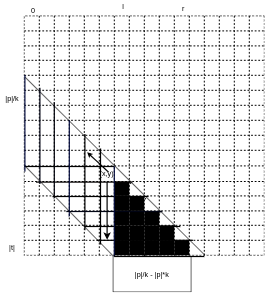
\includegraphics[width=0.4\columnwidth]{figures/M2.png}
   \caption{LOL}\label{M2}
\end{figure}

%The second step, it is one-way pass through these suffixes with a sliding window of size $\frac{|p|}{t}$ to find for each window that has alignment score greater or equal to given threshold $-k_{di}$ with pattern $p$ most similar suffix with the longest length. 



\begin{algorithm}[!t]
\caption{PATTERN BASED NEAR DUPLICATE
SEARCH ALGORITHM VIA SEMI-LOCAL SA}
\label{alg:patternMathing1}
Input: pattern $p$, text $t$, similiarity measure $k \in  [ \frac{1}{\sqrt{3}} ,1  ]$\\
Output: Set of non-intersected clones of pattern $p$ in text $t$
\begin{equation}
    k_{di}=|p|*(\frac{1}{k}+1)(1-k^2)
\end{equation}
\begin{equation}
 L_{w} = \frac{|p|} {k}
\end{equation}
\begin{equation}
  w = |p|(\frac{1}{k} - k)
\end{equation}
Pseudocode:
\begin{algorithmic}[1]
\STATE{$W = semilocalsa(p,t)$}
\COMMENT{1st phase}
\STATE{$H^{str-sub}_{p,t} = semilocalsa(p,t).stringSubstringMatrix$}
\STATE{$M[j,i] = -H^{str-sub}_{p,t}[i,j]  $}
\STATE{$sufixes = processDiagonal(M,L)$}
\COMMENT{2d phase}
\STATE{$W_2 = SuffixMaxForEachWindow(sufixes,L_{w})$}
%% \STATE{$filter(W_2,k_{di})$}
\STATE{ $W_3 = UNIQUE(W_2)$}
\COMMENT{3rd phase unchanged}
\FOR{$w \in W_3$}
\IF{$\exists w^{'} \in W_3:w \subset w^{'} $}
\STATE{ $remove$ $w$ $from$ $W_3$}
\ENDIF
\ENDFOR
\RETURN $W_3$
\end{algorithmic}
\end{algorithm}

\begin{theorem}
Algorithm \ref{alg:patternMathing1} runs in $max(O(|t|*|p|),\ O(|t| * \log |t|))$ time with $O( |t| \log |t|)$ additional space where $p$ is pattern, $t$ is text, $|p| \leq |t|$, and $v=O(1)$ where $v$ is denominator of normalized mismatch score for semi-local sa $w_{normalized} = (1,\frac{\mu}{v},0)$.
\end{theorem}
\begin{proof}
  For each phases of algorithm we provide it's time and space bounds.
  
\emph{First phase.}
We store solution $H$ of \emph{semi-local sa} by decomposing it to permutation matrix $P$ of size $O(v*|t| \times v*|t|)$ (lines 1-3, Theorem~\ref{decomposition}).
The permutation matrix can be stored via two permutations of size $v*|t|$ for columns and rows.
It is simply two lists of size $v*|t|$.
Then, for random access query in specific position $(i,j)$ of matrix $H$ one need to check how many points are dominated by $H [i,j]$.
It can be done by checking all points of permutation matrix and requires $O(v * |t|)$ steps.
Thus, the total time and space complexity of the first phase are $O(v *|p| * |t|)$ (time needed to solve semi-local sa) and $O(v*|t|)$ respectively.
Given $v=O(1)$ we have $O(|p| * |t|)$ and $O(|t|)$ respectively.

\emph{Second phase}.
For the sake of clarity, we omit $k$ factor in algorithm analysis since $k$ is just a constants within interval $(\frac{1}{\sqrt{3}},1]$.

%We proceed diagonal M as follows (\ref{M2}).
First, we query elements that lie in the diagonal that represent
substrings of size $L_{w}=\frac{|p|}{k}$.
Since we can use proposition~\ref{incremental}
The total complexity of this step is $O(|t|)$.
The total amount of querying cells is $O(|t|)$. 
Second, we again process matrix M.
More precisely, we process the diagonal of width $O(\frac{|p|}{k}-|p|*k)=O(|p|)$ that corresponds to all substrings with size in  $I=[|p|*k:\frac{|p|}{k}]$ interval (on Fig. \ref{M2} it is  trapezoid). 

%In the proof, we follow the first approach described in the algorithm description for this phase.
First, we need to access the cell that represents substring $t_{0,|p|*k}$.
Note, such a random access query to a matrix element requires $O(|t|)$ time.
Further, by  proposition~\ref{incremental} we access adjacent elements for given cell $M[i,j]$ by $O(1)$.
Thus, we can traverse through the diagonal of matrix $M$ in time $O(|t|*|p|)$ iteratively as follows.
Let $(i',j')$ denotes the current position.
We process the $i'$-th row starting from position $j'$ until maximum length is reached, i.e. until $i^{'}-j \geq |p|*k$.
% Process row $i^{'}$ with starting $j^{'}$ (recall it cell by $M[i^{'},j^{'}]$) position  (go right i.e increment $j^{'}$) until $i^{'}-j \geq |p|*k$.
When the row is processed we shift by one $i^{'}$ down and $j^{'}$ to right of $(i',j')$ for the next iteration if needed (see \todo{picture} \red{This about the top left corner}).
% Then shift by one $i^{'}$ down and $j^{'}$ to right by one if needed (see picture \red{This about the top left corner}).

Each raw is processed twice.
First, to detect a maximum score.
Second, to find the longest suffix with the highest similarity.
%% When we pass through a slice of the specific row in diagonal $M$,  we also will find the longest suffix with the highest similarity simply by checking elements twice.
%% First for detect maximum score, second for detect the longest suffix among those who have this score.
%It requires storing at most $O(p)$ cells for each column but we only process one column at the time, thus, we will require only $O(p)$ additional space for that whole cell processing.
Thus, for storing for each prefix its longest suffix we need additionally $O(|t|)$ space.
Let $l^{prefs}$ denotes a list of stored prefixes.
Additionally, for each substring of length $\frac{p}{k}$ we store similarity score by querying them during diagonal passage.
Let's denote it by $C$.
Thus, at the end of the diagonal processing (line 4) $O(t)$ suffixes are collected and they require $O(t)$ space for storing.
Hence, the overall diagonal processing (line 4) requires $O(|t|+|t|*|p|) = O(|t|*|p|)$ time with $O(|t|+|p|) = O(|t|)$ additional space.

Further (Line 5), we again traverse each element of list $l^{prefs}$ with one step sliding window of size $L_w$.
For each windows we check wheather it satisfies the similarity criteria, i.e. its similarity score is at most $-k_{di}$.
The check can be performed by a simple lookup for a specific element of $C$ at $O(1)$.
If so then then we need $O(|p|)$ lookups within suffixes to query the most similar and longest one.
%% Further (Line 5), we need to find the longest suffix for each $O(|p|)$ windows with step one in applied to list of size $|t|$ with additional condition that within each window of size $O(\frac{|p|}{k}-|p|*k)=O(|p|)$ the suffix with length $L_{w}$ have similarity score at least $-k_{di}$.
%% It is simply a one-way pass-through list of suffixes where the processing of each window requires at most $O(|p|+1)=O(|p|)$.
%% More precisely, first, we check that for current window of size $O(|p|)$ its associated suffix has similarity not less then given threshold $k_{di}$.
%% It is simply lookup for a specific element in $C$ with $O(1)$.
%% If that true, then we need $O(|p|)$ lookups within $suffixes$ to query the most similar and longest one.
The total number of such windows can be approximated as $O(|t|)$.
Thus, the step (line 5) requires $O(|t|)*O(|p|) = O(|t|*|p|)$ computation time with $O(|t|)$ space.
%% The filtering process (Line 6) is a one-way pass through a list of suffixes $W_2$.
%% It requires at most $O(t)$ time.

Thus, the total running time and space complexity of the second phase is $O(|t|*|p|)$ and $O(|t|)$ respectively.

\emph{Third phase}.
The third phase remains unchanged, thus have the same time and space bounds as in the base algorithm case.
Note, it possible to perform this phase in-place during the second phase which speedups the algorithm, i.e decreases space and time complexity to $O(|t|)$ and $O(|t|*|p|)$ respectively.
The third phase can be approximated as $O(|t| * log|t|)$ for both space and running time complexity.

Thus, the total alforithm running time is $max(O(t * p),\ O(t * \log t))$ while space complexity is $O(t * \log t)$.
%% \red{It be good if we also improve third phase)))}
\end{proof}

\begin{theorem}
Algorithm \ref{alg:patternMathing1} with scoring scheme $w = (0,-2,-1)$ preserves completnesses property of algorithm~\cite{luciv2019interactive} and has running time and space complexity $max(O(t*p),\ O(t* \log t))$ and $O(t *  \log t)$  respectively.
\end{theorem}

\begin{proof}
Edit distance in the base algorithm~\cite{.} may be expressed as sequence alignment with following scoring scheme: 
$$w_{sa}=(w_{+},w_{0},w_{-}) = (0,-2,-1).$$

First, to get intial edit score we need to apply inverse operation:
$$editscore(a,b) = -sa(a,b,w_{sa}).$$
Next, $w_{sa}$ may be normalized using normalization~\ref{weightNormalization}:
$$(0, -2, -1) \rightarrow (1,\frac{\mu=0}{v=1}, 0).$$
\todo{equivalent? Thus, $d_{di} \leq k_{di}$ is the same as $sa \geq -k_{di}$.}

Second, let's carefull review phases 1 and 2 of given algorithms.
The base algorithm passes through the text with a sliding window to detect those fragments of size $L_{w}$ which have edit score above given threshold $k_{di}$.
Then within these fragments algorithm detects longest suffixes that are most similar to pattern $p$ with size within interval \todo{$I=pk...L_{w}$}.
The presented improved algorithm proceeds in a very similar way but, informally, phases are swapped.
First, it detects the longest suffixes with size in interval $I$ for each prefix of the text.
Then, it proceeds in such way that for each window of size $L_{w}$ that has alignment score with pattern $p$ below given threshold $-k_{di}$  the longest suffix most similar to $p$ is detected.
Due to \todo{formula~\ref{editsa}} results of the second phases of the algorithms are equal.
The third phase remains unchaned in the presented algorithm.
%% Thus, the presented algorithm preserves completeness.
Thus, the presented algorithm is complete.
For $w = (0,-2,-1)$, $v=1$ and algorithm running time and space complexity are as claimed.
%% For given $w = (0,-2,-1)$ we have $v=1$ then wehave running time as claimed.
\end{proof}

%At first algorithm \ref{luciv} pass through text $t$ with sliding window to detect those fragments which has similarity abobe given threhsold $k_{di}$ with size $\frac{p}{k}$.
%Then within these fragments algorithm detects longest suffixes most similar to pattern $p$ with size within  $pk...\frac{p}{k}$ interval.
%That how $A_1$ constucted.
%
%T%he second algorithm \ref{alg:patternMathing1} proceed in similar way but it first .
 .
%$Then filtering is perfomed in that way that only$
%That how $A_1$ constucted.
%those lonh suffices  left 
 %for those windows of size $\frac{p}{k}$ the longest suffix is left.

%T%%hus, $A_1=A_2$  by resulting equivalence of construction. 


\section{CutMax a new approximate mathing algorithm}
\label{section:our}
We now describe several algorithms that heavily based on semi-local lcs and it's underlying algebraic structure.

The first algorithm \ref{alg:appximateMatchingGreedy} refers to following constraint.
There should be found all non-intersected clones $\tau_{i}$ of pattern $p$ from text $t$ that has the highest similarity score on the uncovered part of the text $t$ and $l \geq |tau_{i}| \geq r$  i.e algorithm should perform greedy choice at each step with length constraint.
This is a more intuitive approach i.e like looking for the most similar one every time that have enough. 

The algorithm proceeds as follows.
First, semi-local sa problem is solved (Line 1).
Then upon string-substring submatrix of semi-local sa solution is built data structure for performing range queries on it (Lines 2-3).
$IntervalsToSearch$ is structure that holds text intervals where search should be perfomed.
Lines 7-21 corresponds to seaching $interval$ with maximal alignment within the current uncovered part of the text $t_{i,j}$.
More precisely, it refers to searching maximum value with corresponding position (row and column) in submatrix of string-substring $matrix$ within  $t_{i,j}$ (starting at $i$th position and ending at $j$th position of text $t$.
 It is solved via range queries (Line 9).
When detected $interval$ has alignment score less then threshold it means that no clones of pattern $p$ are presented in this part of text $t_{i,j}$, and further processing should be skipped (Line 19).
Otherwise, the founded clone is added to final result and the current part of the text splits on two smaller parts and processed in the same way (Lines 13, 15).
Finally, the algorithm outputs a set of the non-intersected intervals of clones of pattern p in text t.

%Lines 7-21 basically  iterative version of recursion where at each level of recursion amount of quesries is doubles at worst case.
%The total amount of  nodes at each level is following.
%At the bottom level of recursion is $t$ nodes, next level is $t/2$, ith level is $t/2_{i}$.
%Thus, the overall amoount of nodes is $t+\frac{t}{2}+\frac{t}{4}+....1 = t*(1 + \frac{1}{2} + \frac{1}{4}+\frac{1}{2^{i}}) $ = sum.
%As mentioned above complexity of query is O().
%This time complexity of Lines 7-21 is O()....

\begin{algorithm}[H]
\caption{GREEDY-PATTERN BASED NEAR DUPLICATE
SEARCH ALGORITHM VIA SEMI-LOCAL SA}
\label{alg:appximateMatchingGreedy}
Input: pattern $p$, text $t$, theshold value $h$\\
Output: Set of non-intersected clones of pattern $p$ in text $t$\\
Pseudocode:
\begin{algorithmic}[1]
\STATE{$sa = semilocalsa(p,t)$}
\STATE{$matrix = sa.getStringSubstringMatrix() $}
\STATE{$rmQ2D = buildRMQStructure(matrix) $}
\STATE{$intervalsToSearch = \emptyset $}
\STATE{$intervalsToSearch.add((0,|t|)) $}
\STATE{$result = \emptyset$}
\WHILE{$intervalsToSearch.isNotEmpty()$}
\STATE{$i,j = intervalsToSearch.pop()$ }
\STATE{ $interval = rmQ2D.query(i, j, i, j) $ }
   \IF{ $interval.score \geq h $}
   \STATE{ $result.add(interval)$}
   	\IF{$interval.startInclusive - i  \geq 1$}
   	\STATE{$intervalsToSearch.add((i, interval.startInclusive))$}
   	\ENDIF
   	\IF{$j - interval.endExclusive   \geq 1$}
   	\STATE{$intervalsToSearch.add((interval.endExclusive, j))$}
   	\ENDIF
   	
   \ELSE 
   \STATE $continue$ 
   \ENDIF
\ENDWHILE
\RETURN $result$

\end{algorithmic}
\end{algorithm}


The second algorithm \ref{alg:appximateMatchingMax} uses a less sophisticated approach and a more lightweight one but found fewer duplicates of pattern $p$(see example \ref{}).
The algorithm also follows a greedy approach but instead of looking at the uncovered part of text $t$ at each step it looks at the text $t$ and chooses the first available substring with the highest score that doesn't intersect with already taken substrings.
More formally, it approximates algorithm \ref{alg:appximateMatchingGreedy}.

\paragraph{Algorithm description}
First, the \emph{semi-loca sa} problem is solved (Line 1).
Then we solve \emph{complete approximate matching problem} (Line 3) i.e
for each prefix of text $t$ we find the shortest suffix that has the highest similarity score with pattern $p$ (Line 3):
\begin{equation}
    a[j] = \max _{i \in 0 ..j} sa(p,t[i,j]), j \in 0..|t|
\end{equation}

Further, we remove suffixes whose similarity is below the given threshold $h$ (Line 4).
Then remaining suffixes are sorted in descending order (Line 5) and the interval tree is built upon them (Lines 7-11).
The building process comprises from checking that current substring $candidate$ not intersected with already added substrings to $tree$ and adding it to $tree$.
Finally, algorithm output set of non-intersected substrings (clones) of pattern $p$ in text $t$.


\begin{algorithm}[H]
\caption{Greedy approximate}
\label{alg:appximateMatchingMax}
Input: pattern $p$, text $t$, theshold value $h$\\
Output: Set of non-intersected clones of pattern $p$ in text $t$\\
Pseudocode:
\begin{algorithmic}[1]

\STATE{$sa = semilocalsa(p,t)$}
\STATE{$matrix = sa.getStringSubstringMatrix() $}
\STATE{$colmax = smawk(matrix) $}
\STATE{$colmax = colmax.filter(it.score >= h$)}
\STATE{$colmax = colmax.sortedByDescending(it.score)$}
\STATE{$tree = buildIntervalTree()$}
\FOR{$candidate \in colmax$}
\IF{$candidate \cap tree = \emptyset $}
\STATE{$tree.add(candidate)$}
\ENDIF
\ENDFOR
\STATE{$result = tree.toList()$}
\RETURN $result$
\end{algorithmic}
\end{algorithm}

\begin{theorem}
Algorithm \ref{alg:appximateMatchingMax} could  be solved in 
$\max ( O(|p| * |t| * v), O(|t| * \log |t|))$ time with $ O(|t| \log |t|)$ space when $|p|<|t|$ where $p$ is pattern, $t$ is text and $v$ is denominator of normalized mismatch score for semi-local sequence alignment
$w_{normalized} = (1,\frac{\mu}{v},0)$ assuming we are storing solution matrix implicitly.

As shown in section \ref{section:preliminaries} the time complexity 
of solving $semi-local sa$ is $O(|p|*|t|*|v|)$ respectevely.
The space complexity of storing monge matrix of semi-local solution is
$O(|t| * v * \log {|t| * v })$ at most due to fact that $v-subbistochastic matrix$ has at most $v$ non-zeros in each row and upon $v * |t|$ points we 
build range tree data structure that \red{??}.

$SMAWK$ algorithm requires $O(|t|*q)$ time where $q$ stands for time complexity of  random access of monge matrix.
Thus, the  total time complexity of line 3 is \red{$O(|t|*?)$ }.
Filtering and sorting have at most $O(|t|)$ and $O(|t|log|t|)$ time complexity.
In Line 6 simple intialization of interval tree is perfomed.   
 
 

\end{theorem}


\begin{corollary}
Algorithm \ref{alg:appximateMatchingMax} could  be solved in 
$\max ( O(|p| * |t|), O(|t| * \log |t|))$ when $v = O(1)$.
\end{corollary}

\begin{corollary}
Algorithm \ref{alg:appximateMatchingMax} could  be solved in 
$ O(|p| * |t| * v )$ when  and amount of clones is small.

When amount of clones is relatively small and threshold value is set high  then after filtering out $t$ intervals (Line 4) sorting is perfomed on s small set of elements.
Thus this part is dominated by calculating semi-local sa solution.
\end{corollary}




\begin{theorem}
Algorithm \ref{alg:appximateMatchingGreedy} could  be solved in 
$\max ( O(|p| * |t| * v), O(|t| * \log |t|))$ time with $ O(|t| \log |t|)$ space when $|p|<|t|$ where $p$ is pattern, $t$ is text and $v$ is denominator of normalized mismatch score for semi-local sequence alignment
$w_{normalized} = (1,\frac{\mu}{v},0)$.

On the first phase of alg

The first phase of algorithm requires $O(|p| * |t| * v)$ with $O(|t| * v)$ additional space for stroring monge matrix implicitly.
We denote this matrix, specifically it's lower-left quadrant that refers to
string-substring solution as $M$ with size $|t| \times |t|$.


  Theorema 3.4
First, note that 

Building structure for rmq queries for staircase matrix requires 
Theorem 5.8. Given an n × n partial Monge matrix M, a data structure of size O(n) can be con-
structed in O(n logn) time to answer submatrix maximum queries in O(log logn) time.
   

\red{Proof it}
\begin{displaymath}
    D = \diag(d_1,\dots,d_n)
  \end{displaymath}
\end{theorem}


\begin{corollary}
Algorithm \ref{alg:appximateMatchingGreedy} could  be solved in 
$\max ( O(|p| * |t|), O(|t| * \log |t|))$ when $v = O(1)$.

\end{corollary}




  

%Given some rope $t$ and small rope $p$ you need to make cuts to form small ropes $t_{i_{1},j_{1}},t_{i_{2},j_{2}}...,t_{i_{k},j_{k}}$ for some $k$ and select some of them that very similiar to  rope $p$ i.e have high similiarity score.
%For that, we would consider constarint that each select of $t_{k} = t_{i_{k},j_{k}}$ should be made greedy i.e   $t_{k}$ it has the highest similiarity score against $p$ over all possible choices of      

 
%The following interpretation can be applied.
%Given text interval $t_{i}$   
%\section{Evaluation}
\label{section:evaluation}

\subsection*{Semi-local algorithms}
Show perfomance between lcs and semi-local lcs??? and poor perfomance of recursive algorithm based on steady ant?

\subsection*{Approximate matching algorithms}
Show outperforming for different cases between luciv and our algorithm.

Show quality betwee our new algo and  luciv algo (our should be better)

Show that sparse table bad when large?
 

\section{Conclusion}
\label{section:conclusion}

Say may be succesfully be applied on practice (showed by algorithm luciv updated)


Open problem.$->$

Say that need to implement with monge2020 (what we not finished)

Improve algo based on recursive steady ant. Because it's critical for algos based on it.


% df\cite{GoVa13}

%% \section*{Acknowledgments}
%% We would like to acknowledge the assistance of volunteers in putting
%% together this example manuscript and supplement.

\bibliographystyle{siamplain}
\bibliography{references}
\end{document}
